%%%%%%%%%%%%%%%%%%%%%%%%%%%%%%%%%%%%%%%%%%%%%%%%%%%%%%%%%%%%%%%%%%%%%%%%%%%%%%%%%%%
%%Anna University sample latex thesis format for UG thesis
%--------------------------------
%%This is the main file that includes the front matter and other chapter links. 
%%Chapters are placed within the folder named 1, 2,...  
%%To compile, run the command `pdflatex authesis.tex' in the terminal. 
%%Some packages may not be needed. Comment the ones, that are not needed. 
%%Images can be saved in the format of *.png. 
%%------------------------------------------------------
%% Authors:
%%Originally used by Dr. Mary Anita Rajam and then modified by Dr. Bama Srinivasan according to the latest Anna University regulations. %%Please report changes to bama@annauniv.edu, chorse@gmail.com %%
%%Acknowledgement: Thanks to Dr.Ranjani Parthasarathi, who relentlessly and patiently guided Bama Srinivasan.
%---------------------------------------------------------
%% Modification added:
%%new file apalikem is added, which gives a neat reference list with 1, 2...
%%aureportm has appendix starting with Arabic numbers
%% Disclaimer: Check with the latest Anna University regulations before working with this format.
%% Changes as on July 2016 
%% 1. Changed the appendix back to alpha mode in aureport.cls
%% 2. Table of contents - reduced the top margin and spacing
%% 3. Added the counter depth for sections to 4 in aureport.cls
%% 4. Deleted chapter number, title and page number in TOC
%% 5. Reduced the top space in chapter titles from 6.5 cms to 5.5 cms in aureport.cls
%% 6. Changes in references use the package natbib and style unsrt. Include a .bib file for the bibliography
%$$$$$$$$$$$$$$$$$$$$$$$$$$$$$$$$$$$$$$$$$$$$$$$$$$$$$$$$$$$$$$$$$$$$$$$$$$$$$$$$$$$$$$$$$$

\documentclass[13 pt,a4paper]{aureportm}
\usepackage{mathptm}\usepackage{etex}
\reserveinserts{28}
\renewcommand{\normalsize}{\fontsize{13 pt}{14.6 pt}\selectfont}
%\usepackage{aunatbib}
%\usepackage{apalikem}
\usepackage{natbib}
\usepackage{bussproofs} % for deduction rules 
\usepackage{auphd}
\usepackage{array}
\usepackage{tabularx}
\usepackage[none]{hyphenat}
\usepackage[chapter]{algorithm}
\usepackage{algpseudocode}
\usepackage{multirow}
\usepackage{multicol}
\usepackage{float}
\usepackage{booktabs}
\usepackage{amsmath}
\usepackage{amssymb}
\usepackage{amsthm}
\usepackage{latexsym}
\usepackage{verbatim}
\usepackage{ifthen}
\usepackage{graphicx}
\usepackage{hyperref}
\usepackage{epsfig}
\usepackage{pslatex}
\usepackage{setspace}
\usepackage{titlesec}
\usepackage[subfigure]{tocloft}
\usepackage{subfigure}
\usepackage{longtable}
\usepackage{enumerate}
\usepackage{lscape}

\usepackage[format=hang,labelfont=bf,textfont=bf]{caption}
\PassOptionsToPackage{linktocpage}{hyperref}
\tocloftpagestyle{myheadings}
\newcommand{\PreserveBackslash}[1]{\let\temp=\\#1\let\\=\temp}
\let\PBS=\PreserveBackslash

\usepackage{colortbl}
\usepackage{newlfont}


\newboolean{psoutput}
\setboolean{psoutput}{true}
\usepackage{pst-all}
\newcommand{\defname}[1]{\emph{#1}.}

\newtheorem{fact}{Fact}[chapter]

\floatstyle{ruled}
\newfloat{algorithm}{htp}{loa}
\floatname{algorithm}{Algorithm}


\titleformat{\section}[hang]{\bfseries}{\makebox[20mm][l]{\thesection}}{0pt}{}{}
\titleformat{\subsection}[hang]{\bfseries}{\makebox[20mm][l]{\thesubsection}}{0pt}{}{}



 \newcounter {definition}[chapter]
\renewcommand \thedefinition {\arabic{chapter}.\arabic{definition}}
\newenvironment{definition}
{ \refstepcounter{definition}
   {\noindent \bf Definition \arabic{chapter}.\arabic{definition}.}}
 {}
 \def\enddefinition{$\Box$}

 \newcounter {example}[chapter]
 \renewcommand \theexample
 {\arabic{chapter}.\arabic{example}}
 \newenvironment{example}
 { \refstepcounter{example}
   {\noindent \bf Example \arabic{chapter}.\arabic{example}.}}
 {}
 \def\endexample{$\Box$}

 \newcounter {proposition}[chapter]
 \renewcommand \theproposition {\arabic{chapter}.\arabic{proposition}}
 \newenvironment{proposition}
 {\refstepcounter{proposition}
   {\noindent \bf Proposition \arabic{chapter}.\arabic{proposition}. }}
 {}
 \def\endproposition{$\Box$}

\pagenumbering{roman}
\setcounter{page}{3}
%\setcounter{secnumdepth}{3}
\renewcommand{\baselinestretch}{1.5}
\newcommand{\row}{i}
\newcommand {\combined} {{C}}
\newcommand {\mtis} {}

\newboolean{showalter}
\setboolean{showalter}{true}
\newcommand{\alter}[1]{\ifthenelse{\boolean{showalter}}{ \{ #1 \} }{}}
\providecommand{\tabularnewline}{\\}
\newcommand{\bigsize}{\fontsize{15pt}{20pt}\selectfont}

\author{Author of the thesis}


\renewcommand{\cfttoctitlefont}{\bfseries\Large}
\renewcommand{\cftlottitlefont}{\bfseries\Large}
\renewcommand{\cftloftitlefont}{\bfseries\Large}


%\cftsetindents{chapter}{0mm}{10mm}
%\cftsetindents{section}{10mm}{10mm}
%\cftsetindents{subsection}{20mm}{10mm}
%\setlength{\cftbeforechapskip}{1.2\baselineskip}
%\setlength{\cftbeforesecskip}{.8\baselineskip}
%\setlength{\cftbeforesubsecskip}{.8\baselineskip}
%\setlength{\cftbeforefigskip}{.8\baselineskip}
%\setlength{\cftbeforetabskip}{.8\baselineskip}
%
\makeatletter
\renewcommand{\@dotsep}{10}
\makeatother
\renewcommand{\cftdot}{ }
\cftsetrmarg{1.2in} % changed by bama - earlier it was 1.5 inch. right margin is decreased to 1 inch.

\titleformat{\section}[hang]{\bfseries}{\makebox[20mm][l]{\thesection}}{0pt}{}{}
\titleformat{\subsection}[hang]{\bfseries}{{\thesubsection}}{0pt}{}{}
\titleformat{\subsubsection}[hang]{\normalsize\bfseries}{\makebox[20mm][l]{\thesubsubsection}}{0pt}{}{}
\titleformat{\paragraph}[hang]{\normalsize\bfseries}{\makebox[20mm][l]{\theparagraph}}{0pt}{}{}
\titleformat{\subparagraph}[hang]{\normalsize\bfseries}{\makebox[20mm][l]{\thesubparagraph}}{0pt}{}{}

\begin{document}

\pagenumbering{roman}


\thispagestyle{empty}
\begin{center}
  \LARGE
  \textbf{\uppercase{Technical Debt Identification Using Text Classification}} \\
  \vspace{0.2\baselineskip}
  \bigsize{\textbf{PROJECT REPORT}}\\
 \vspace{0.4\baselineskip}

  \normalsize{\textit{\textbf{Submitted by}}}\\
  \vspace{0.5\baselineskip}
  {
  \Large \textbf{Kaliappan}}\\
  %\normalsize{\textbf{(Roll number)}}\\
  \Large{\textbf{David Sundaraj}}\\
  \Large{\textbf{Prashanth Lidwin Jessuva}} \\
   \vspace{0.6\baselineskip}
  %\normalsize{\textit{A report for the phase-I of the project}}\\
  \vspace{-0.1\baselineskip}
  \normalsize{\textit{submitted to the Faculty of}} \\
  \vspace{0.5\baselineskip}
  \normalsize{\textbf{INFORMATION SCIENCE AND TECHNOLOGY}} \\  
  \vspace{1\baselineskip}
  \normalsize{\textit{in partial fulfillment  for the award of the degree}}\\
  \normalsize{\textit{\textbf{of}}}\\
\vspace{.2\baselineskip}
  \bigsize{{\textbf{BACHELOR OF TECHNOLOGY}}}\\
  \normalsize{\textit{\textbf{in}}}\\
  \bigsize{{\textbf{INFORMATION TECHNOLOGY}}}\\
\end{center}
  \begin{center}
   %
\includegraphics[width=26mm,height=25mm]{auemblem.pdf}   \\
   
\includegraphics[scale=0.5]{auemblem.pdf} \\
  \normalsize{ \textbf{DEPARTMENT OF INFORMATION SCIENCE AND TECHNOLOGY }}\\
  \normalsize{\textbf{COLLEGE OF ENGINEERING, GUINDY}}\\
  \normalsize{\textbf{ANNA UNIVERSITY}}\\
  \normalsize{\textbf{CHENNAI  600 025}}\\
  \vspace{0.01\baselineskip}
  \normalsize{\textbf{MONTH YEAR}}
 \end{center}
\pagebreak

\chapter*{ANNA UNIVERSITY\\
CHENNAI - 600 025\\
%\vspace{\baselineskip}
BONA FIDE CERTIFICATE}
\newlength{\aulength}
\settowidth{\aulength}{Anna University
  Chennai}
\newlength{\datewidth}
\settowidth{\datewidth}{Chennai 600 025}

\begin{spacing}{1.5}
  \begin{sloppypar}
  \fontsize{13}{14.5}\selectfont Certified that this project report titled Technical Debt Identification Using Text Classification is the bona fide work of Kaliappan, David, Prashanth who carried out project work under my supervision. Certified further that to the best of my knowledge and belief, the work reported herein does not form part of any other thesis or dissertation on the basis of which a degree or an award was conferred on an earlier occasion on this or any other candidate.
  \end{sloppypar}
\end{spacing}
\vspace{-0.3 cm}
\begin{flushleft}
 \parbox[t]{\datewidth}{\small{\textbf{PLACE:\,CHENNAI}}\\
 \small{\textbf{DATE:\, 31/11/2018 }}}
 \hfill
 \parbox[t]{6 cm}{\small{\textbf{Dr. SASWATI MUKHERJEE}} \\
 \small{\textbf{PROFESSOR}}\\
 \small{\textbf{PROJECT GUIDE}}\\
 \small{\textbf{DEPARTMENT OF IST, CEG}}\\
 \small{\textbf{ANNA UNIVERSITY}}   \\
 \small{\textbf{CHENNAI  600025}}
 }
\end{flushleft}
%\vspace{0.5 cm}
\begin{center}
 \small{\textbf{COUNTERSIGNED}}\\ 
  \vspace{1.5 cm}
  \textbf{\small{Dr. SASWATI MUKHERJEE}}\\ 
  \small{\textbf{HEAD OF THE DEPARTMENT}}\\
 \small{\textbf{DEPARTMENT OF INFORMATION SCIENCE AND TECHNOLOGY}}\\
 \small{\textbf{COLLEGE OF ENGINEERING, GUINDY}}\\
 \small{\textbf{ANNA UNIVERSITY}}   \\
 \small{\textbf{CHENNAI  600025}}
 
\end{center}



%\addtocontents{toc}{\protect\flushleft \protect\bfseries
%CHAPTER NO. \hfill TITLE \hfill PAGE NO.\endgraf}

%\addtocontents{toc}{\protect\raggedleft Page\\}

 %\addtocontents{lof}{\protect\flushleft
%\protect\bfseries FIGURE NO. \hfill
% TITLE \hfill  PAGE NO.\endgraf}%
%\addtocontents{lot}{\protect\flushleft \protect\bfseries TABLE NO. \hfill
%  TITLE \hfill  PAGE NO.\endgraf}%


\chapter*{\uppercase{ABSTRACT}}
\addcontentsline{toc}{section}{\bfseries \uppercase{Abstract}}

The issue of Technical debt has been a subject of controversy for sometime now, Technical debt as such is not harmful for a software project but it is essential to identify such technical debts in the project as soon as possible because the later you find the more the debt increases and at last it becomes unbearable to pay back similar to the financial debts in our real life.
\par There have been many methods suggested to identify technical debts in the project like Code Smells, Source Code Analysis, Comment analysis etc., In this project we have come with a new and novel way to identify these technical debts and it is by going through the bug reports of that particular software. On applying text processing to the bug reports we have classified a bug report as either a technical report or a non-technical report. Thus the developers and testers can concentrate in detail on the bugs that were marked as technical.
\par For this project we have concentrated on the Chromium Project, it is a open source project from Google. The bug can be filed by anyone using a software called Monorail. We have scraped 700 of these issues for now as our dataset and given this to software engineering experts who classified these bugs as either technical or non-technical. This is the dataset using which we have experimented with various Text Classification methods. In essential we are using NLP methods to analyse and understand the issues and then classify it as either Technical or Non-Technical.
\par \emph{Keywords}: Technical Debt, Chromium Project, Code Smells, NLP.

\chapter*{\uppercase{ACKNOWLEDGEMENT}}
%\addcontentsline{toc}{section}{\bfseries \uppercase{Acknowledgement}}
We would like to thank our HOD for having faith in us and giving us this project to work on and we would like to thank her for her guidance and support. We also thank Dr.Prabhavathy who helped us to understand things when HOD is busy with a work. We also thank our project lab professor Dr.Sridhar for giving us some valuable advice and guiding us in this project.

\setlength\cftparskip{0pt}
\setlength{\cftbeforetoctitleskip}{-3em} %Decrease the top margin of toc title
%\setlength{\cftaftertoctitleskip}{0 em} 
\setlength{\cftbeforelottitleskip}{-3em} % Decrease the top margin of lot
\setlength{\cftbeforeloftitleskip}{-3em} % Decrease the top margin of lof
\cftsetindents{chapter}{0 mm}{10 mm}
\cftsetindents{section}{10 mm}{10 mm}
\cftsetindents{subsection}{20 mm}{10 mm}
\cftsetindents{subsubsection}{30 mm}{15 mm}
\cftsetindents{paragraph}{40 mm}{20 mm}
\cftsetindents{subparagraph}{50 mm} {20  mm}
\cftsetindents{table}{10 mm}{10 mm}
\cftsetindents{figure}{10 mm}{10 mm}
%%%%%%%%%%%%%%%%%%%%%%%%%%%%%%%%%%%%%%%%%%%%%%%
%Changes made as on June 2016
%%%%%%%%ADD TOC with one half spacing%%%%%%%%%%%
\begin{onehalfspacing} 
\tableofcontents

%\clearpage
\end{onehalfspacing}
%%%%%%%%%%%%%%%%%%%%%%%%%%%%%%%%%%%%%%%%%%%%%%
% These are old as of April 2016 -
%%%%%%%%%%%%%%%%%%%%%%%%%%%%%%%%%%%%%%%%%%%%%%%%
%\cftsetindents{chapter}{0.2in}{1.5in}
%\cftsetindents{section}{1.7in}{0.3in}
%\cftsetindents{subsection}{1.8in}{0.4in}
%\cftsetindents{table}{0.2in}{1.5in}
%\cftsetindents{figure}{0.2in}{1.5in}
%\tableofcontents



%\pagebreak

%\addcontentsline{toc}{section}{\bfseries LIST OF TABLES}
%\listoftables
% \clearpage \addcontentsline{toc}{section}{\bfseries
%LIST OF FIGURES} \listoffigures
%\clearpage
%%%%%%%%%%%%%%%%%%%%%%%%%%%%%%%%%%%%%%%%%%%%%%%%%%%%%%%%%%%
\chapter*{LIST OF SYMBOLS AND ABBREVIATIONS}
\addcontentsline{toc}{section}{\bfseries LIST OF SYMBOLS AND ABBREVIATIONS}

\setlongtables
\begin{longtable}
  {>{\PBS\raggedright\hspace{0pt}}p{3cm}@{}%
    >{\PBS\raggedright\hspace{0pt}}p{11.5cm}@{}}

  %$A$ & Set of attributes\\ 
  %$a_t$ & Time attribute\\
  $-$, $\neg$, $\sim$  & Negation operator \\
  $+$, $\vee$, $\cup$ & Disjunction operator \\
  $X$, $\wedge$ & Conjunction operator \\
  $\rightarrow$ & Conditional operator \\
  $\leftrightarrow$ & Biconditional operator \\
  $\diamond$ & Future tense modal operator\\
  $\alpha$ & Action \\    
  \end{longtable}
%\end{tabular}

%\clearpage

%\newpage
\pagenumbering{arabic}

\ausection
% Chapter 1

\chapter{\uppercase{Introduction}} % Main chapter title
\label{intro} % For referencing
\section{\uppercase{Motivation:}}
Technical Debt is a shortcut taken in a project development which is taken in order to speed up the delivery or completion of the project. Technical Debt as such is not harmful for example not commenting important information in some parts of the code and releasing it in a hurry is also a form of technical debt but the very crucial thing is after it is delivered the development team must make sure that they go back to the released skeleton and make sure that they comment it as soon as they get time after releasing the first version.
\par The real problem kicks in when after releasing the project if the team still does not add the left out comments, then future development of this code is hampered. So technical debt causes a problem when we let the debt to accumulate very similar to Financial Debt, in finance we make sure that the Debt we borrowed does not reach a humongous proportions, if it reaches such levels then we will not be able to pay off our Debts. Similarly if we do not periodically monitor and pay back our Technical Debts then it causes a huge disaster for companies.
\par But Technical Debt is not always identifiable, because sometimes by accident a Technical Debt is formed, so it is very hard to identify a Technical Debt in a software project.So it is becoming very important and pertinent for many companies around the world in the present to identify a very efficient and accurate method to identify a Technical Debt in a software project. Finding a accurate method which detects Technical Debt is the motivation of our project.
\section{\uppercase{Project Background:}}
For our project we are working on the Chromium Dataset that we got from Penn State University. Chromium is the open source counterpart of Google Chrome and the dataset are the bug issues of the browser Chromium, and there is a need for Chromium project to find out the bugs that have Technical Debt inherent with them, this is necessary because a bug due to Technical Debt causes a big software disaster and hence those bugs must be identified as soon as possible. At present Chromium project makes use of Software engineering experts to identify the Technical Debt bugs.
\par Chromium project has a open source issue tracker from where this data is extracted. Our Dataset consists of 700 issues out of which 200 issues are classified by software engineering experts and remaining 500 issues are classified by CMU. All 700 issues can be seen in the Issue-Tracker. We also have scraped out some issues from the issue tracker for our project. The 700 issue dataset has a binary classification label- either label T which indicates the description is Technical or NT which indicates that the issue is Non-Technical.
\par The dataset that we got has the following fields: Id, Author, Comments, Comments-Date, Comments-Label, Date, Description, Role, Status, Title, Type, Closed, Priority, Rating, Date, Label and Keywords. So we are applying our NLP and ML logic on this dataset.
\section{\uppercase{Necessity:}}
\begin{itemize}
\item At present the issues are being classified by Software Engineering experts. It takes a lot of time and money as it involves human Labour. 
\item Labelling each issue involves looking into a great amount of data about that issue which can be overwhelming.
\item So it is necessary that inorder to fasten this process there is need to automate this labelling process, for this we need to come up with a algorithm that reads a issue and then gives it a label which is as accurate as given by a human expert.
\end{itemize}
\section{\uppercase{Challenges:}}
\begin{itemize}
\item No one has tried this method of automating this process
\item We have to find a suitable feature selection method that will help in classification of these documents.
\end{itemize}

% Chapter 2

\chapter{\uppercase{Literature Survey/Related Work}} % Main chapter title
\label{ch:survey} % For referencing

In order to understand about technical debt and the current methods of identifying this in a project there was an extensive Literature Review done, as part of the Literature Review many IEEE and ACM papers were read so that there is a complete understanding about the existing methods and the places where the method can be improved.
\section{\uppercase{The WyCash portfolio management system.}}
In the development of a software named WyCash+ for Wyatt Technology, there was a problem of a new feature fitting poorly in existing architecture, by using a makeshift method the new feature was accommodated and released. Later this makeshift method was replaced with the fully functional feature. Cunningham had first used the analogy of “technical debt” in this research paper.
\section{\uppercase{Tracking Technical Debt.}}
In this paper the authors had monitored a real MNC application. The application they monitored made use of MS-Exchange Server. At the time when they started work on this application the latest version of MS Exchange Server they had was 2003 version and there was the news that MS Exchange Server 2007 was going to release sooner or later, but they started developing the project with dependency on MS Exchange 2003. But unfortunately within 6 months of release the project MS Exchange 2007 version got released and hence they had to scrape out the released software thus causing a huge loss for the MNC. 
\section{\uppercase{Technical debt and agile software development practices and processes.}}
Agile software development process and practices have an effect on technical debt. Agile practices safeguarding software implementation have the most positive effect. Technical debt knowledge is implicit and hence the concept is under utilised.
\section{\uppercase{Identifying Self-Admitted Technical Debt in Open Source Projects Using Text Mining.}}
In this paper the authors made use of text mining to identify self admitted technical debt. Self admitted technical debt is the technique of adding information about technical debts in source codes by adding comments etc., Like for example someone may comment saying that “they have added a temporary variable as a shortcut” etc., Thus on mining these comments we must identify whether it happens to be a Technical Debt or not. They have made use of natural processing techniques in order to identify the Technical Debts in the source file.
\section{\uppercase{Detecting Technical Debt from Issue Trackers.}}
In this paper the authors made use of text mining on the issues that are found in the Issue trackers of the software. For this paper the authors had used the issues of a particular software whose issue can be got from the issue tracker. And then using a key word approach they extracted features and then gave it to Naive Bayes Classifier and thus got the required results.

% Chapter 3

\chapter{\uppercase{Design of your work}} % Main chapter title
\label{ch:chap3} % For referencing
Your actual work should come in here. Include system architecture, modules, etc., with diagrams and provide an explanation for each of these.  
\section{\uppercase{View of Tables}}
Sample view  is shown in Table \ref{tab:first} and an example is given in Table~\ref{tab:second}.
\begin{table}[h]
\caption{Example 1}
\begin{center}
\begin{tabular}{|c|c|}
\hline
$c1$ & $c2$ \\
\hline
r1 & r2 \\
\hline
r1  & r2 \\
\hline
\end{tabular}
\end{center}
\label{tab:first}
\end{table}
\begin{table}[h]
\caption{Example 2}
\begin{center}
\begin{tabular}{|c|c|}
\hline
\textit{x} & \textit{y}  \\
\hline
\textit{x} & \textit{not y}  \\
\hline
\end{tabular}
\end{center}
\label{tab:second}
\end{table}

\section{\uppercase{View of Figures}}
Examples of pictures are shown in Figure \ref{fig:one} and Figure \ref{fig:two}.
\begin{figure}[h]
\begin{center}
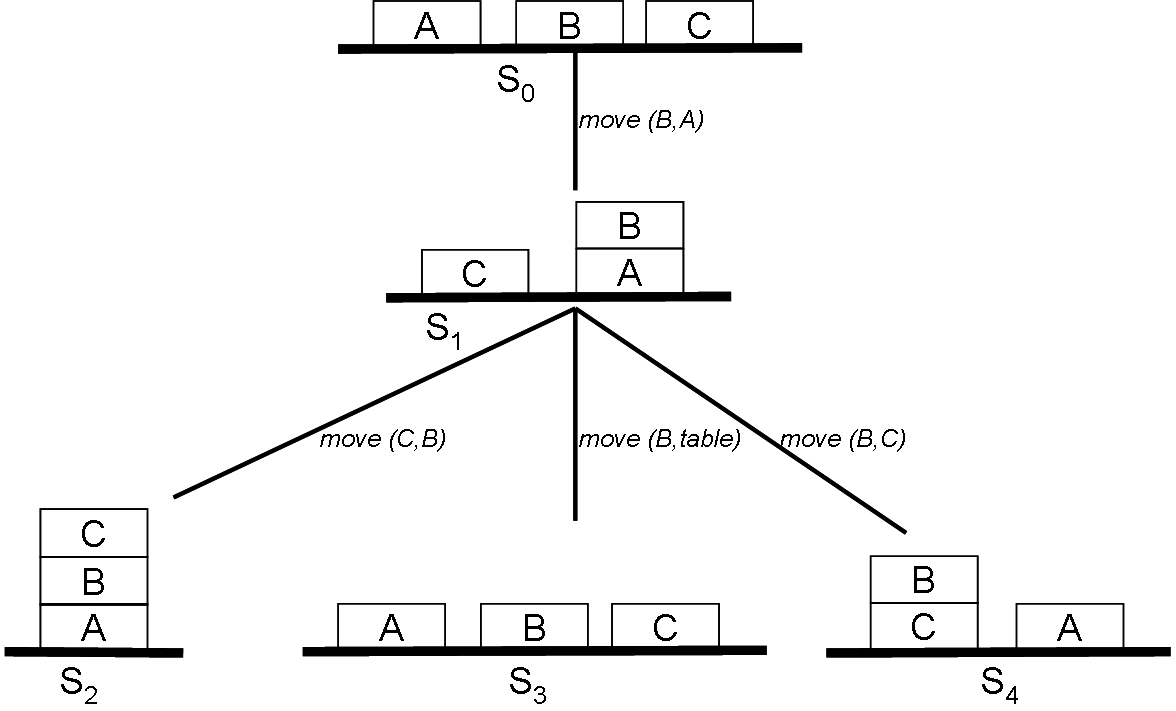
\includegraphics[scale=0.6]{3/eg1.png}
\caption{Example 1}
\label{fig:one}
\end{center}
\end{figure}
\begin{figure}[h]
\begin{center}
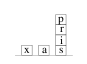
\includegraphics[scale=2]{3/eg2.png}
\caption{Example 2}
\label{fig:two}
\end{center}
\end{figure}

\section{\uppercase{View of Equations}}
The sum of squares of $a$ and $b$ are calculated as shown below:
\begin{eqnarray}
 \label{eq:sum}
 (a+b)^2 = a^2+b^2+2ab
\end{eqnarray}

From Equation \ref{eq:sum}, the data is obtained.






% Chapter 4

\chapter{\uppercase{Implementation of your work}} % Main chapter title
\label{chap4} % For referencing
The implementation details of your work should be mentioned in this chapter.
\section{\uppercase{Algorithm 1}}
\begin{algorithm}
\begin{algorithmic}[1]
\State Get the number of variables $num$ 
\State Start with an empty list $x$ $[~]$
\For {each $n$ of $num$}
	\State Get the $x$
	\State  Get the $t$
	\State Get the $w$
\EndFor 
\If {$xl$ == $s$} 
	\State terminate with the failure message \textbf{failed}
\Else
	\State $z = x$
\EndIf 

\end{algorithmic}
\end{algorithm}




% Chapter 5

\chapter{\uppercase{Modules:}} % Main chapter title
\label{chap5} % For referencing
\section{\uppercase{Module 1:}}
Initially we are going to do a trial and error process where we will try out as many NLP methods and at the same time try out as many Machine learning techniques like classification, prediction etc., Then we are trying to mix Machine learning and NLP feature selection technique. Initially we are working by taking only the Description and Label fields of the Dataset. Then we are going to try the Ensemble methods to see their classification acuracy. So in the second major part we will be making use of the other fields that are available in the dataset.

\section{\uppercase{Module 2:}}
In this phase we will try and finish the Semi-Supervised Learning Method. Then we are planning to do a social network analysis of the creators and moderators of the particular issue, and we are going to include their social networking behaviours to the classification process, So that essentially we give importance to the comments of the people who are really technical people and not some non technical people who may have some less insight into the real nature of the bug.
%% Chapter 6

\chapter{\uppercase{Comparison}} % Main chapter title
\label{chap6} % For referencing
This chapter is optional. Depending on the work, comparison can also be included in previous chapter.


\chapter{\uppercase{Conclusion and Future Work}}
\label{chap:conclusion}
We found that out of the current features and classification methods the ensemble method proves to give the highest accuracy. Now for future work we must and try and improve the feature selection method that we are using in this project. And then test and see how the feature selection method improves the accuracy.
\cleardoublepage
\phantomsection 


%\bibliographystyle{auapalike}
\bibliographystyle{unsrt}
\nocite{*}%This gives a list of all references that includes without citation. Remove this, once the reference is cited
\phantomsection
\addcontentsline{toc}{chapter}{REFERENCES}
\begin{spacing}{1}
\bibliography{publication}
\end{spacing}

\newpage
\clearpage




\addtocontents{toc}{\protect\newpage}
\addtocontents{lot}{\protect\newpage}
\addtocontents{lof}{\protect\newpage}

\end{document}
